% -*- coding: utf-8 -*-

\section{Rectangular Swept Spheres}
\label{rss}

\subsection{Introduction}
In this section I will go into greater detail about the RSS, how it is defined and represented, as well as the literature that I have used in this report. I will also shortly describe Oriented Bounding Boxes (OBB), Point Swept Spheres (PSS), and Line Swept Spheres (LSS). No other bounding volumes will be described or used in this report.

\subsection{Rectangular Swept Sphere}
The Rectangular Swept Sphere (RSS) is a 3D figure. It is generated by sweeping the center of sphere over a rectangle in 3 dimensional space. This makes it resemble a rectangular rounded pillow. An illustration of a RSS can be found in figure \ref{rss-example-figure} on page \pageref{rss-example-figure}. 

\subsection{Representation of RSS}
I have chosen to represent the RSS as a rectangle in 3D, a radius, as described in \cite{larsen00fast}, \cite{Larsen99fastproximity} and \cite{237244}, and with a OBB, in order to be able to quickly do an Axis-separation test. The rectangle is represented by 2 vectors, a center point. See section \ref{rectangle3d} page \pageref{rectangle3d} for  implementation details. I felt this was best way to represent it, as it describes a RSS while using a minimum of memory, and follows the representation found in \cite{237244}, which enables me to use the axis-separation test described in \cite{237244}.

\begin{figure}
\centering
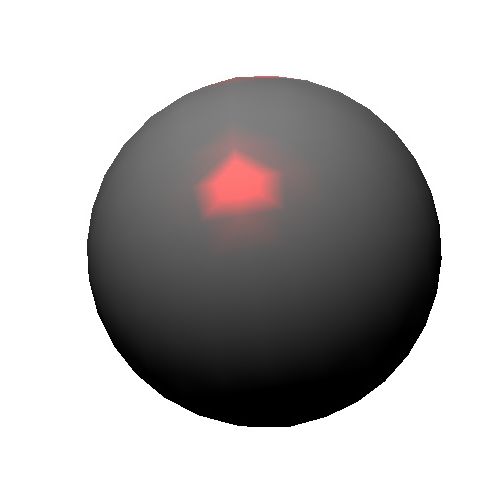
\includegraphics[width=0.5\textwidth]{figures/pss}
\caption{\label{pss-example}An example of a PSS}
\end{figure}

\subsection{Point Swept Spheres}
A point swept sphere is a BV that is created by taking a point p in 3D, and placing the center point of a sphere at p. The advantage of the PSS is that it is both simple to implement and to do an overlap check with other PSS. However, PSS' can easily get a bad fit, as the only adjustable properties that can be adjusted are the radius and the location of the center point.

\begin{figure}
\centering
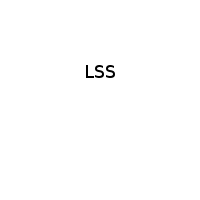
\includegraphics[width=0.5\textwidth]{figures/lss}
\caption{\label{lss-example}An example of a LSS}
\end{figure}

\subsection{Line Swept Spheres}
A line swept sphere is a BV that is created by sweeping the center point a sphere across a line-segment. It is a bit harder to check for overlap in LSS' than PSS' (see above), but since proteins are often spirally formed, LSS will often in practice have a better fit than PSS', and will therefore perform fewer checks, possibly making it more effective.

\begin{figure}
\centering
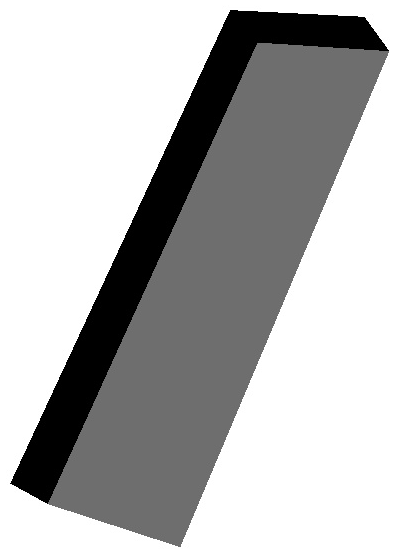
\includegraphics[width=0.5\textwidth]{figures/obb}
\caption{\label{obb-example}An example of a OBB}
\end{figure}

\subsection{OBB}
The Oriented Bounding Box is a Box with a height, width and length, and a orientation. For an example of an OBB, see figure \ref{obb-example}. As I will explain later, RSS' and OBB's based on the same point set should have a similar volume - with the RSS in most cases having a volume that is slightly larger, at least if implemented naively.

\subsection{Literature used in this report}
\label{lit}
For this project I have used the following literature:
\begin{description}
\item[\cite{larsen00fast}] Gives an introduction on how to perform a fast distance query between RSS' with a pruning method that eliminates at least half of the tests. The article only gives a brief overview of the pruning method, the reasoning behind it and how to perform it in practice, and refers to \cite{Larsen99fastproximity} (by the same authors) for more detail. There is also a brief description of an alternative method to the Axis-separation used in this project, to detect whether 2 RSS' overlap, where the authors uses the slabs defined by 2 points. The slab-method seems like it could be far more effective than the Axis-separation test, but I have not attempted to implement it, as it is not described in any great detail, and comes after a reference to \cite{Larsen99fastproximity}, making it seem like an afterthought.   

\item[\cite{Lotan03algorithmand}] Gives a general introduction to Monte Carlo simulation of Proteins, as well as a comparison of several BV's and the algorithms for these, for protein folding. Nothing in \cite{Lotan03algorithmand} is used directly, but rather as background material for the domain.

\item[\cite{Larsen99fastproximity}] Gives an more in-depth exploration of the minimum distance calculations mentioned \cite{larsen00fast}, as well as an overview of the method they have used to generate the RSS' using OBBs. While the explanation of the pruning method both convincing and implementable, the authors does not explicitly explain a case that the authors mention ``needs extra analysis for closest point test'' (\cite{Larsen99fastproximity} section 4.3.1, page 14), but is not further elaborated upon. \cite{Larsen99fastproximity} also tries to explain the slab-method mentioned in \cite{larsen00fast} in greater detail, but the structure of the explanation makes it possible for the reader to think that the authors has used the Axis-separation method for their solution, in order to check whether the 2 RSS' are separated or not. The description of the slab-method itself is also not very specific, and does not explicitly mention the radius property of the RSS further muddling the water as the radius property is central, instead the authors prefer to focus on the case where the rectangles of the RSS' are overlapping.

\item[\cite{237244}] Gives a description of the axis-separation test for OBB's, as well as a description on how to optimize the checks. The entire process is well explained.
\end{description}

\subsection{Conclusion}
I have in this section described the Rectangular Swept Sphere, as well as the 3 other BV that I that I will work with throughout this report. I have furthermore given an example of all 4 BVs, and gives a short critique of the main literature I have used for this project.
